\section{The Tabu search method}
\subsection{Description of Tabu search methods}
Tabu search is a heuristic optimization method designed to find the global optimum. The algorithm has the ability to climb out of a local minimum, and then explore other parts of the domain. There are several methods on how this abilitiy can be acquired. Tabu search uses a so-called tabu list, intended to make already visited areas in the domain forbidden (``tabu''). Tabu searchalgorithms are based on certain conseptual buildingblocks and basic ideas. Most of them are easy to understand but widely varying in difficulty to implement. If well implemented they will give you a highly sofisticated search algorithm. \\
\\The main buildingblock is the tabu list. The tabu list gives the algorithm the ability to render certain regions or moves tabu. The tabus can be created based on the information at hand, both for a given moment and from prior experiences of the search. The essential problem when constructing tabu search algorithms is about to formulate intelligent rules, that will determine is a specific move should be tabu or not.\\
\\Another important buildingblock is the tabu overriding mechanism, in literature this is usually named as the aspiration criteria. The aspiration criteria checks whether a certain move should be approved, even if it initially was set to be tabu. \\
\\With these two methods buildingblocks one can construct almost any type of logical structure. This makes the tabu search method highly implementable and adaptive. The tabu search method is stocastic, meaning that the tabu list and aspiration criteria only deals with randomly selected solutions. This means that the current solution is not necessarily a good one. One of the strengths of the tabu search algorithms is that \emph{any solution produced tells something about the problem at hand, independent of the solutions' quality.} In practice this means that a bad solution also yields important information.  Or, to quote Thomas Edison 
\begin{quotation}
\emph{``I have not failed 1,000 times.  I have
successfully discovered 1,000 ways to NOT make a light bulb.''}
\end{quotation}
This insight might seem somewhat naive at first sight, but if implemented in a good way it yields powerful results.
%skall laggas in I ordbeskrivnings kappitlet\\
%Word convention:\\ 
%Complete solution = a set of moves that have solved the problem.\\
%Incomplete solution = a set of moves that will not solve the problem.\\
%Feasible solution = a set of moves that have not yet solved the problem, or have not yet been evaluated whether it is a complete/incomplete solution.\\
%fitness evaluation...something like genetic
\begin{figure}[!h]
	\centering
	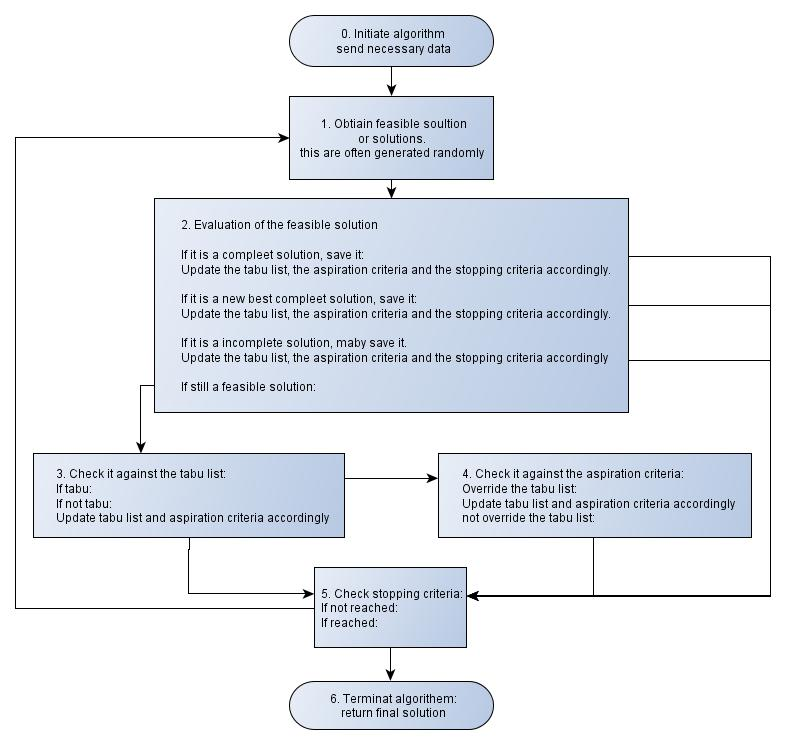
\includegraphics[width=\textwidth]{chapter_4_methods/tabu_generell.jpg}
  	\caption[Generic flow chart of tabu algorithm]
  	{Flow chart of tabu algorithm}
\end{figure}

\subsection{Development process of the Tabu search algorithm}
The developement process of the tabu search algorithm for our problem will here be described in detail. One of the restrictions of this project was that it had a time shortage due to a deadline. Because of this the alternatives that were easiest to implement was usually prefered. The development process originated from a general flowchart of the algorithm, given in figure 4.2. By following the flow chart, in step one we arrive at the first issue to resolve. The issue of whether to construct a set of feasible solutions, or one single feasible solution at a time. Since the genetic algorithm already had implemented a way of constructing sets of feasible solutions, it was decided to construct one feasible solution at a time.\\
\\
Two alternatives on how to construct this single feasible solution was considered. Either by generating the feasible solution one pursuer step at a time, or by a series of steps. It was decided to construct the feasible solution with one pursuer step at a time. This was a hard decission to make, since both alternatives seemed to yield highly promising but very different algorithms. The implementation of making a series of moves would result in a receding horizon approach, where one had to either  
\begin{itemize}
\item[-]{}Produce a large set of series of moves. Sort these by fitness, then choose one to check against the tabu list and aspiration critera.
\item[-]{}Generate a single series of moves to check against the tabu list and aspiration critera.
\end{itemize}
The implementation of this approach would require that the tabu list and aspiration critera had abilities of a more analysing type. This implied that it would be very difficult to implement within the given time.\\
\\This settled we can now move on to discuss the ideas that form the tabu list. Seven different rules where considered, presented below.
\begin{enumerate}
\item{}For one feasible solution save the past X number of moves for each pursuer and render these moves tabu to be returned to.
\item{}Do not allow moves that results in X number of lost secured tiles.
\item{}Make geometricaly based tabus for critical areas:\vspace{0,1cm}\\
A corridor where the end point can be seen should not be walked down by a pursuer. Also, a region with an obstacle that can be circulated would need two pursuers to be secured. Thus it would be tabu to go about and try to secure it alone. And finaly if one hade a tree like corridor system, going about to solve it would only be allowed with the right amount of pursuers.
\item{} Work togheter. \vspace{0,1cm}\\
Two pursuers never really need to see each other, only share vissible areas. Since this rule is general in its formulation it should be called upon in the aspriation criteria.
\item{} High valued areas \vspace{0,1cm}\\
Tiles walked upon in a complete solution should be given a value bonus. Or implemented differently, tiles not walked upon could be set to be tabu. This is an attempt to incorporate the idea of getting information even from bad, but complete, solutions.
\item{} Low valued areas \vspace{0,1cm}\\
Some tiles that are part of an incomplete solution are probable to be of low interest. Hence these tiles could be given a penalty.
\item{} Treading in secured areas is not probable to yield promising results. Thus this should be given a penalty, or not allowed.
\end{enumerate}

All these tabu rules are to be ranked and given a priority level that would be used in the aspiration criteria. Also many of the tabu rules listed above needed some sort of worst case senario handeling, in order to avoid that the algorithm would freeze.\\
\\We will now discuss the aspiration critera. As understood from the tabu rules presented above a lot is to be incorporated in the aspiration critera. It needs to have the ability of checking whether a tile is of high or low value.

Which in turn means that the\textbf{ evaluation steps } in figure [4.2] needs a fitness calculation function that would depend on the tile visited and the shape of the feasible solution. Unfortunately this aspiration criteria would need an overwhelming amount of work to implement. Thus this advanced aspiration criteria was rejected for a simpler one. In the end the more simple aspiration criteria only came to be a worst case handling, to avoid the algorithm from freezing. This also means that tabu rules (3), (4), (6) and (7) no longer could be implemented. Tabu rule (5) got simplified to: tiles not walked upon where set to be tabu.\\
\\A comment on tabu rule (5) is that when this rule first was implemented the idea was that X number of past complete solutions were analysed to check which areas had been walked upon at least once, and render the rest tabu. The problem was however that this wasn't strict enough, so X was set to one. Which in turn led to a new problem. The problem that arouse was that the algorithm now, under certain circumstances, was too hasty in returning a final solution. This was partially solved by a new stopping criteria and a ``go about it again'' criteria.\\
\\The final version of the algorithm can be viewed in figure [4.3 ] and is also presented in the next section.
\subsection{The Tabu search algorithm for our problem}
%kollat hit!
%kollat hit.
%kollat hit.
%kollat hit.
%kollat hit.
The tabu search algorithm used for solving the problem be discussed here.\\
In figur [generella tabu] a generall step by step explanation was made of the tabu search algorithm. In figur [???] a modified version can be seen, intended to illustrate the final algorithm and also to show what functions from to the general algorithm that was removed.\\

\begin{figure}[!h]
	\centering
	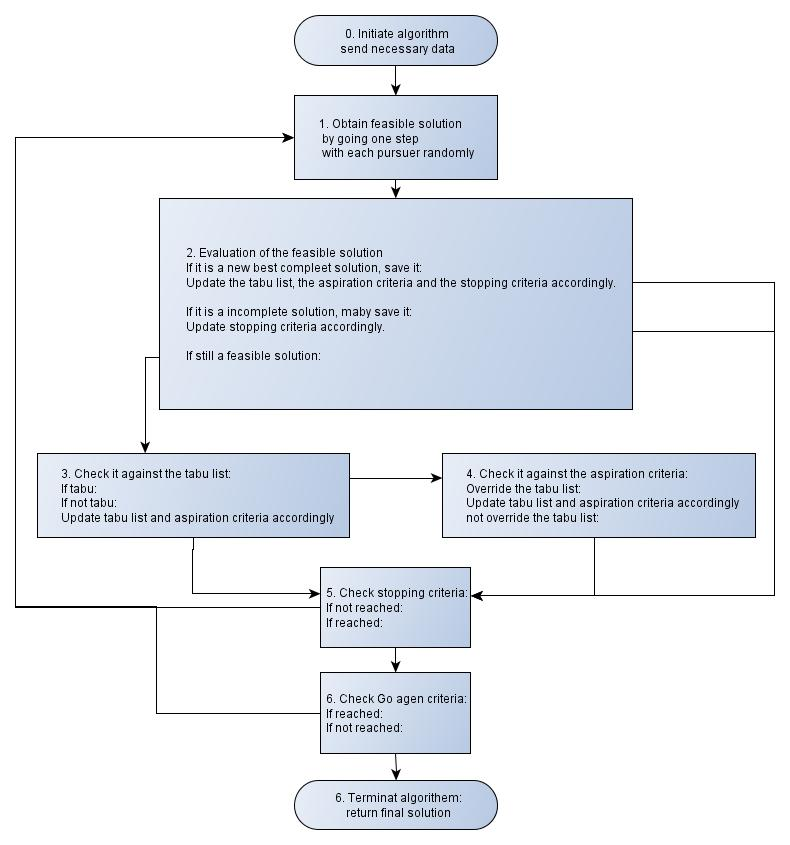
\includegraphics[width=\textwidth]{chapter_4_methods/tabu_ny.jpg}
  	\caption[Final algorithm flow chart of tabu algorithm]
  	{Final algorithm flow chart of tabu algorithm}
\end{figure}

To get a feel for the algorithm and to point out insufficiencys, an explanation of how the algorithm converges is in order.\\
There are two elements in the algorithm that affect the convergens:
\begin{enumerate}
\item{} Tabu roule (5)
\item{} Best-solution-found-so-far stopping criteria. \vspace{0,1cm}\\
Mening that if a solution is found one does not search for a solution with a path of longer length.
\end{enumerate}
To note here is that both convergens helping elements depend on that they actualy hava a complete solution. Meaning that if the algorithm is unlucky in finding the first complete solution, the computational time will rise acordingly. As a said note, this considerable insufficiency migth have been avoided with the more advansed aspiration critera, discussed in section [develupment].

\subsection{Implementation of the Tabu search algorithm}
In this section two important aspects of the implementation will be discussed. These two are obvious shortcomings in the algorithm and parameter values. With the implementation, a series of parameter values arouse. Parameter values that had three different features:
\begin{enumerate}
\item{} Tabu rule values:
\begin{enumerate}
\item{} Tabu rule (1)  save\_past\_X\_number\_of\_moves 
\item{} Tabu rule (2)  X\_number\_of\_lost\_secured\_areas
\end{enumerate} 
\item{} Aspiration criteria values:
\begin{enumerate}
\item{} Override\_X\_number\_of\_lost\_secured\_areas
\item{} Override \_save\_past\_X\_number\_of\_moves
\end{enumerate} 
\item{} Stopping criteria values:
\begin{enumerate}
\item{} Max\_incomplete\_solutions\_ found \_in\_a\_row
\item{} Max\_ equal\_complete\_solutions\_ found \_in\_a\_row
\item{} Max\_allowed\_steps
\end{enumerate} 
\item{} Go again values:
\begin{enumerate}
\item{} Restart\_the\_algorithm\_X\_times
\item{} Restart\_the\_algorithm\_X\_times\_keep\_best\_complete\_solution
\item{} X\_steps\_is\_this\_realy\_the\_best\_complet\_solution
\end{enumerate} 
\end{enumerate} 
As can be seen in the list above some of the parameters have strong relations to eachother. These relations will now be explained. \\
Parameter values (1) and (2) are related in a way so that (2) ensures that (1) does not make the algorithm freeze. \\
Parameter value (4b) and (4c) aims to avoid the algorithm from being to hasty in returning a final solution, when encountering a less difficult enviroment. The Max\_allowed\_steps and Restart\_the\_algorithmen\_X\_times tries to tackle the problem of finding the first complete solution. The computational time, and the probability of finding any solution at all, totally depends on this relation. As discussed lastly in section 4.2.3 the algorithms' computational time will be affected if the first complete solution is found at a late stage in the search. But the computational time will be even greater affected if one wants to increase the probability of finding a solution at all. Meaning that if The Max\_allowed\_steps value is increased, the chances of finding a complete solution should increase. \\
Parameter value (3a) and (3b) has two properties, first to terminate the algorithm and secondly to not terminate the algorithm until the search space has been throughly examined in promising regions. Parameter (3b) is also an indicator of that the the search has converged to a certain final solution.\\
\\
\indent Obvious shortcomings in the algorithm:\\
Mera text
1. kan inte st� still
2.  
